\documentclass[12pt]{article}

\usepackage{amsfonts, amsmath, amssymb}
\usepackage[backend=biber, style=apa]{biblatex}
\addbibresource{.bib}

\usepackage{enumitem}

\usepackage{graphicx} % Required for inserting images
\graphicspath{ {images/} }

\usepackage{caption}
\usepackage{subcaption}

\renewcommand{\figurename}{Fig.}

\usepackage{ragged2e}

\usepackage{xcolor}
\usepackage{listings}

\usepackage{xparse}

\usepackage{dcolumn}

\usepackage{etoolbox}
\makeatletter
\patchcmd{\@verbatim}
  {\verbatim@font}
  {\verbatim@font\scriptsize}
  {}{}

\usepackage{sectsty}

\definecolor{LightGray}{gray}{0.9}
\definecolor{DarkGray}{gray}{0.2}

\NewDocumentCommand{\code}{v}{%
\texttt{\fontsize{11}{12}\selectfont\setlength{\fboxsep}{2pt}\colorbox{LightGray}{\textcolor{DarkGray}{#1}}}%
}
\renewcommand{\maketitle}{\begin{titlepage}
    \begin{center}
        \vspace*{1cm}
            
        \Huge
        \textbf{ ST1131 Assignment 2}
            
        \vspace{0.5cm}
            
        \vspace{1.5cm}

        \LARGE
        Chin Zhe Ning, A0255895J
            
        \vfill
            
        \Large
        National University of Singapore\\
        April 2023
            
    \end{center}
\end{titlepage}}
\usepackage[a4paper, margin=0.83cm]{geometry}

% edits for submission
\sectionfont{\normalsize}
\subsectionfont{\normalsize}
\subsubsectionfont{\small}

\usepackage{draftwatermark}
\SetWatermarkText{A0255895J}
\SetWatermarkScale{5.2}
\SetWatermarkLightness{0.98}
\SetWatermarkAngle{0}

\begin{document}

\maketitle
\pagestyle{empty}

\section{Introduction}

This report proposes a linear regression model to predict the resale price of HDB flats in Singapore, based on a dataset of transactions from 2012. The model will consider factors such as location, floor area, flat model, and storey range. We acknowledge that the data's relevance to today's market may be limited due to changes in inflation, housing policy, and socioeconomic factors. The report will provide an overview of the dataset, describe the methodology used to develop the model, present the results, and discuss its strengths and limitations.

\section{Data characteristics}
The dataset is obtained from \url{https://data.gov.sg/dataset/resale-flat-prices}, it is uncertain whether the data is randomized but we will assume the case for the analysis.
\begin{figure}[!htp]
    \centering
    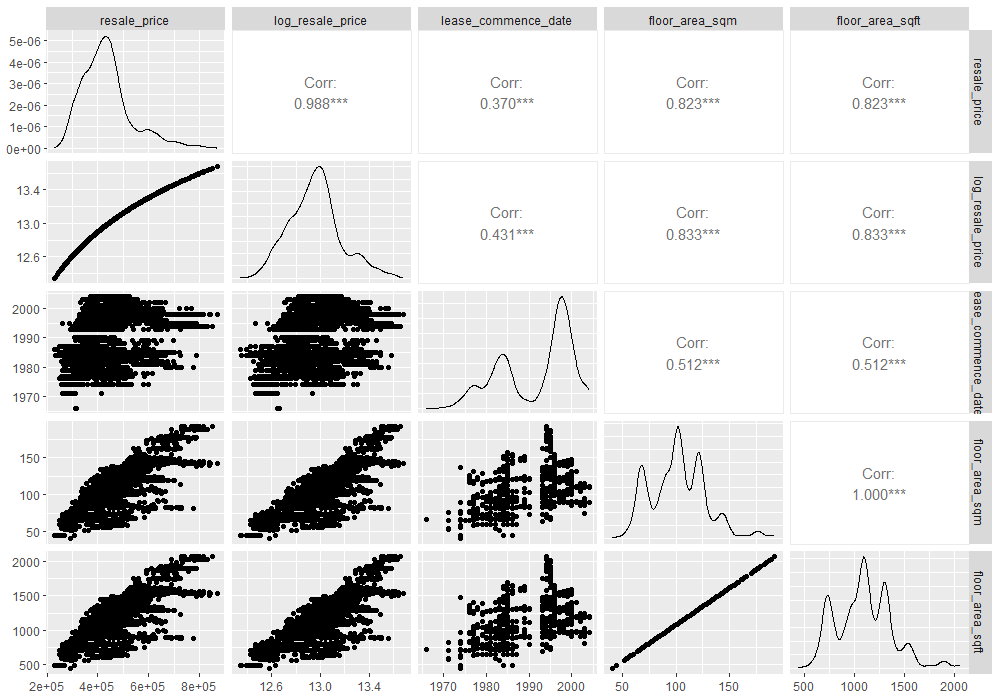
\includegraphics[width=0.7\textwidth]{images/scatterplotmatrix.png}
    \caption{Scatterplot matrix of quantitative variables.}
    \label{fig:scatterplot matrix}
\end{figure}

We observe that \code{resale_price} is quantitative which is necessary for regression modelling and the distribution is right-skewed. There is weak or no correlation between \code{lease_commence_date} and \code{resale_price} as shown by the low correlation of 0.370 so we will not consider \code{lease_commence_date}as a regressor. There is a strong linear correlation between \code{floor_area_sqm} and \code{resale_price}.
\begin{verbatim}
    > head(street_name)
    [1] "ROWELL RD"   "ROWELL RD"   "CHANDER RD"   "TG PAGAR PLAZA"   "QUEEN ST"   "KLANG LANE"
    > length(unique(street_name))
    [1] 66
\end{verbatim}

Note that \code{street_name} has many categorical variables that are not well distributed. In our analysis, we found categories with very few observations, such as ``Jlm Berseh" with 3 observations only. The inclusion of \code{street_name} in the model may lead to overfitting or increased variability of the estimated coefficients. Hence, we will not consider \code{street_name} as a regressor.

\section{Model Selection and Interpretation}

\subsection{Preliminary Models}
Before arriving at the final model, we considered several preliminary models. In this section, we describe each of these models, including the choice of transforms, interactions, and regressors. We also discuss the reduction of non-significant regressors that informed the selection of the final model.

\subsubsection{Initial Model}
The initial model is a simple linear regression model with a logarithm transform for the response variable \code{resale_price}. The systematic component consists of the explanatory variable \code{floor_area_sqm}.

As we identified from our preliminary analysis, \code{resale_price}, is right-skewed, hence we apply a logarithm transform to \code{resale_price} to achieve a more symmetrical distribution. This is necessary for \code{resale_price} to be suitable for linear regression. Since \code{resale_price} is large, boundary conditions will be avoided, hence the transform is appropriate. The histograms of \code{resale_price} before and after the transform are shown in Fig. \ref{fig:histogram_transform}.

A high correlation value of 0.833 between \code{log(resale_price)} and \code{floor_area_sqm} was also observed. Therefore, we expect \code{floor_area_sqm} to be a significant predictor of \code{resale_price}.

\begin{figure}
\centering
\begin{minipage}[t]{0.73\textwidth}
    \centering
    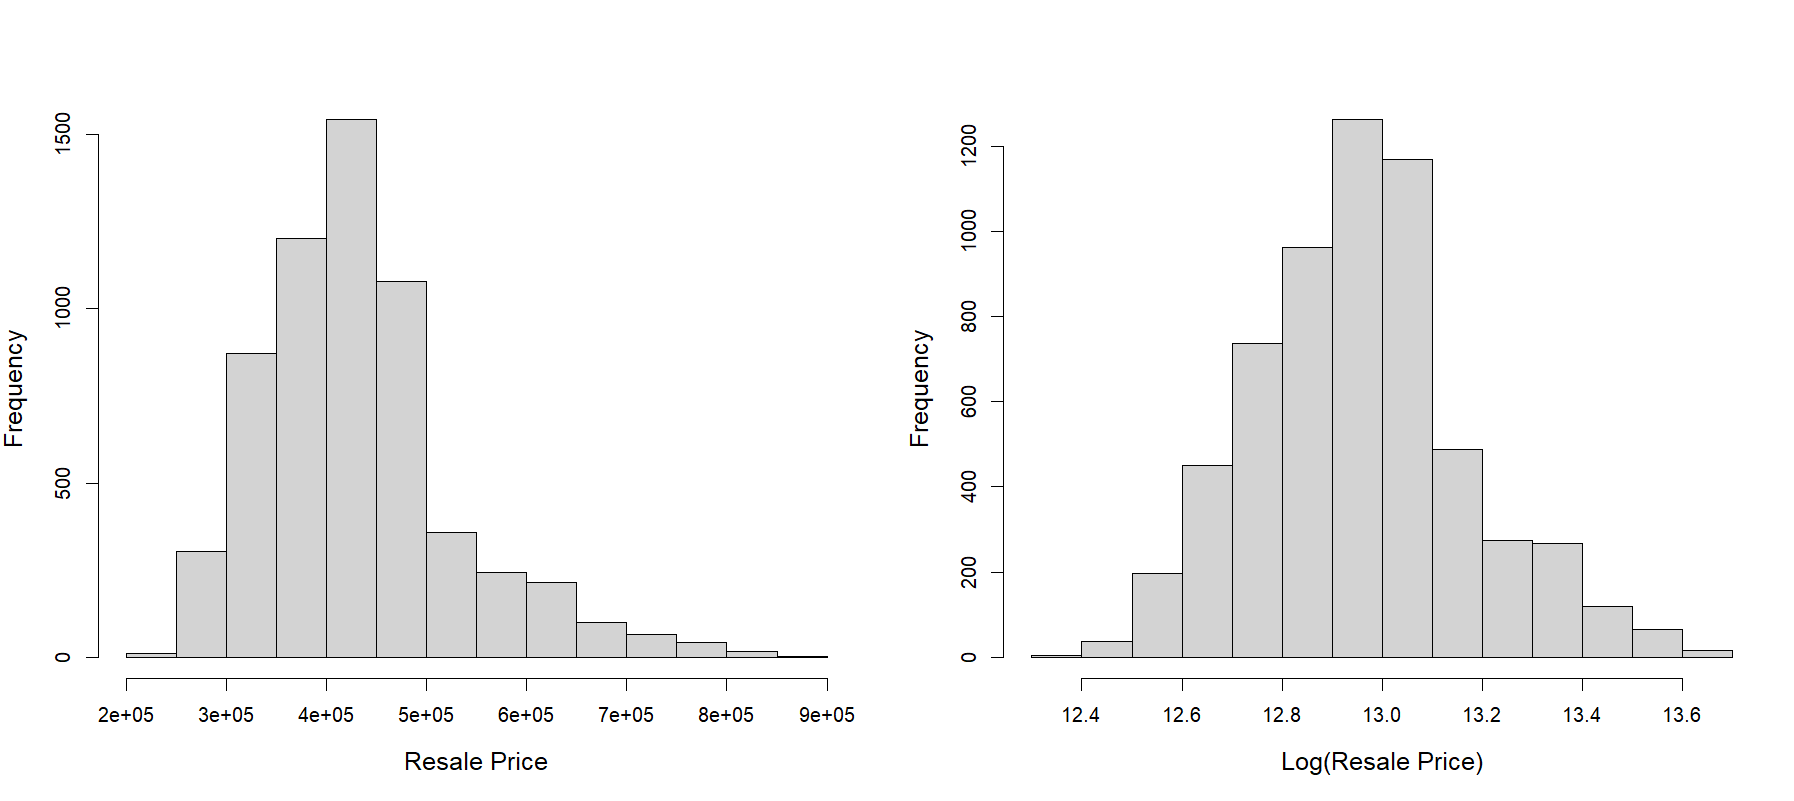
\includegraphics[width=\textwidth]{images/Screenshot 2023-04-11 175624.png}
    \caption{Histogram of resale\_price before and after logarithm transform.}
    \label{fig:histogram_transform}
\end{minipage}\hfill
\begin{minipage}[t]{0.26\textwidth}
  \centering
  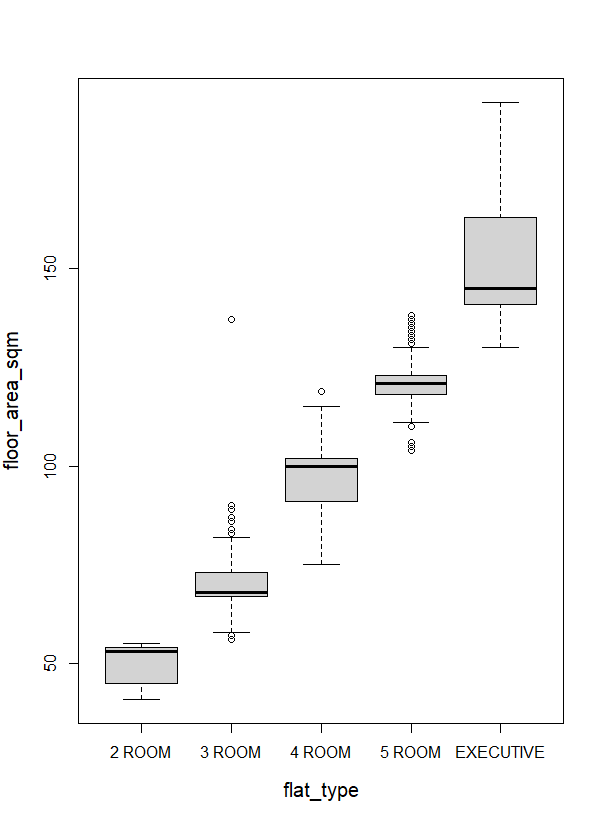
\includegraphics[width=\textwidth]{images2/floor_area_sqm against flat_type.png}
  \caption{floor\_area\_sqm against flat\_type.}
  \label{fig: boxplot}
\end{minipage}
\end{figure}

\begin{figure}
    
\end{figure}

To check for linearity, \code{log(resale_price)} is plotted against \code{floor_area_sqm} (Fig. \ref{fig: m1 plotted}) A clear and strong linear association is observed.

Verifying these assumptions, we then proceed with the model specification:
\[M_1: \log(\text{resale\_price}) \sim \text{floor\_area\_sqm}\]
where \code{log(resale_price)} is the log-transformed response variable, the resale price of HDBs, and \newline \code{floor_area_sqm} is the explanatory variable representing the floor area of the HDB flat in square meters ($m^2$).

This model was then fitted in R with the \code{lm()} function using the Ordinary Least Squares (OLS) Method. The model summary is provided in Fig. \ref{fig: m1 model summary}.

\begin{figure}[!htp]
\centering
\begin{minipage}[t]{0.45\textwidth}
  \centering
  \caption{$M_1$ Linear Regression Line}
  \label{fig: m1 plotted}
  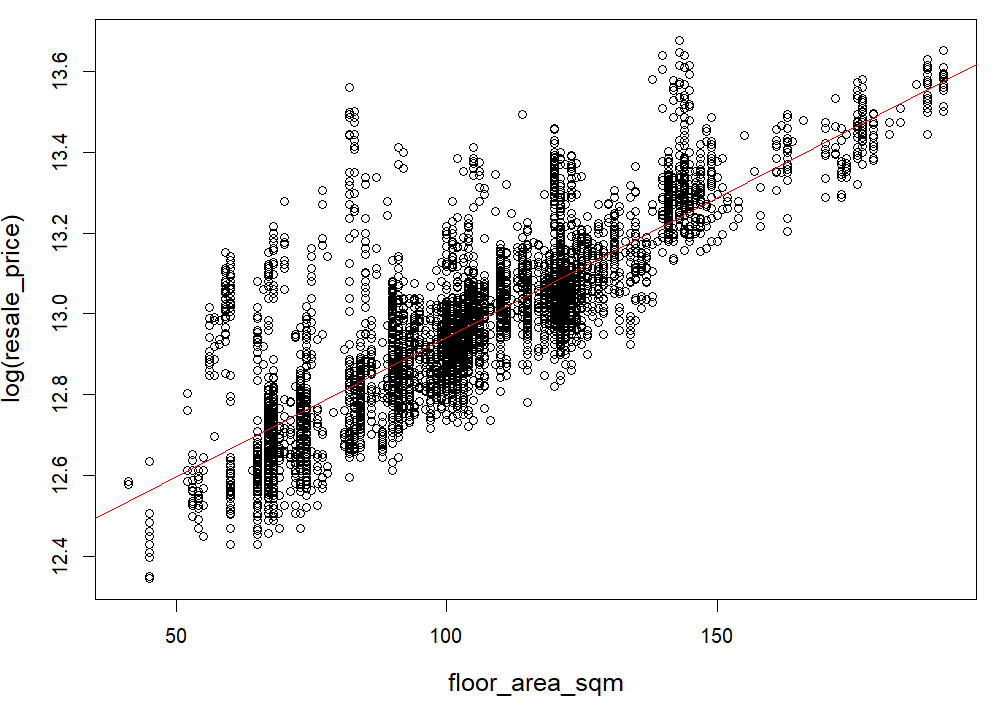
\includegraphics[width=\textwidth]{images/Screenshot 2023-04-11 201739.png}
\end{minipage}\hfill
\begin{minipage}[t]{0.49\textwidth}
  \centering
  \caption{$M_1$ Model Summary}
  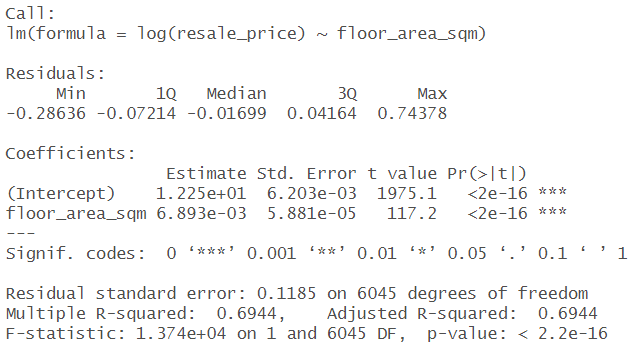
\includegraphics[width=\textwidth]{images/Screenshot 2023-04-11 201612.png}
  \label{fig: m1 model summary}
\end{minipage}
\end{figure}


The fitted equation for $M_1$ is $\log(\text{resale\_price}) = 0.006893 \times \text{floor\_area\_sqm} + 12.252$. This shows that for every increase in floor area ($m^2$), there is an increase of 0.006893 in log resale price. Note that the p-value of the F-test ($< 2.2 \times 10^{-16}$) is very small, and indicates that the overall model is statistically significant. This is of no surprise as \code{log(resale_price)} and \code{floor_area_sqm} are highly correlated. However, the $R^2$ value (0.694) is not very high, so the $M_1$ does not have strong predictive power. This suggests that the model has poor goodness of fit. The model also has a residual standard error of 0.119 on 6045 degrees of freedom.

We now check the normality assumption. From the normal QQ-plot of the standardised residuals (SR) for $M_1$ (Fig. \ref{fig: m1 res plot and qq plot}), we see that the quantile points are not consistent with the theoretical normal line as the right-tail deviates. This means that the SR do not follow a normal distribution. 

We also check for constant variance. The residual plot (Fig. \ref{fig: m1 res plot and qq plot}) of $M_1$ shows that the spread of the variance varies across the fitted values. For higher fitted values, there is a lower spread present as seen from the funnel shape. This suggests that constant variance is not present. Both the normality and constant variance assumption are not satisfied, therefore, $M_1$ is not accurate and cannot be used. The next step is to introduce more explanatory variables to improve the accuracy and goodness-of-fit of $M_1$.

\begin{figure}[!htp]
\centering
    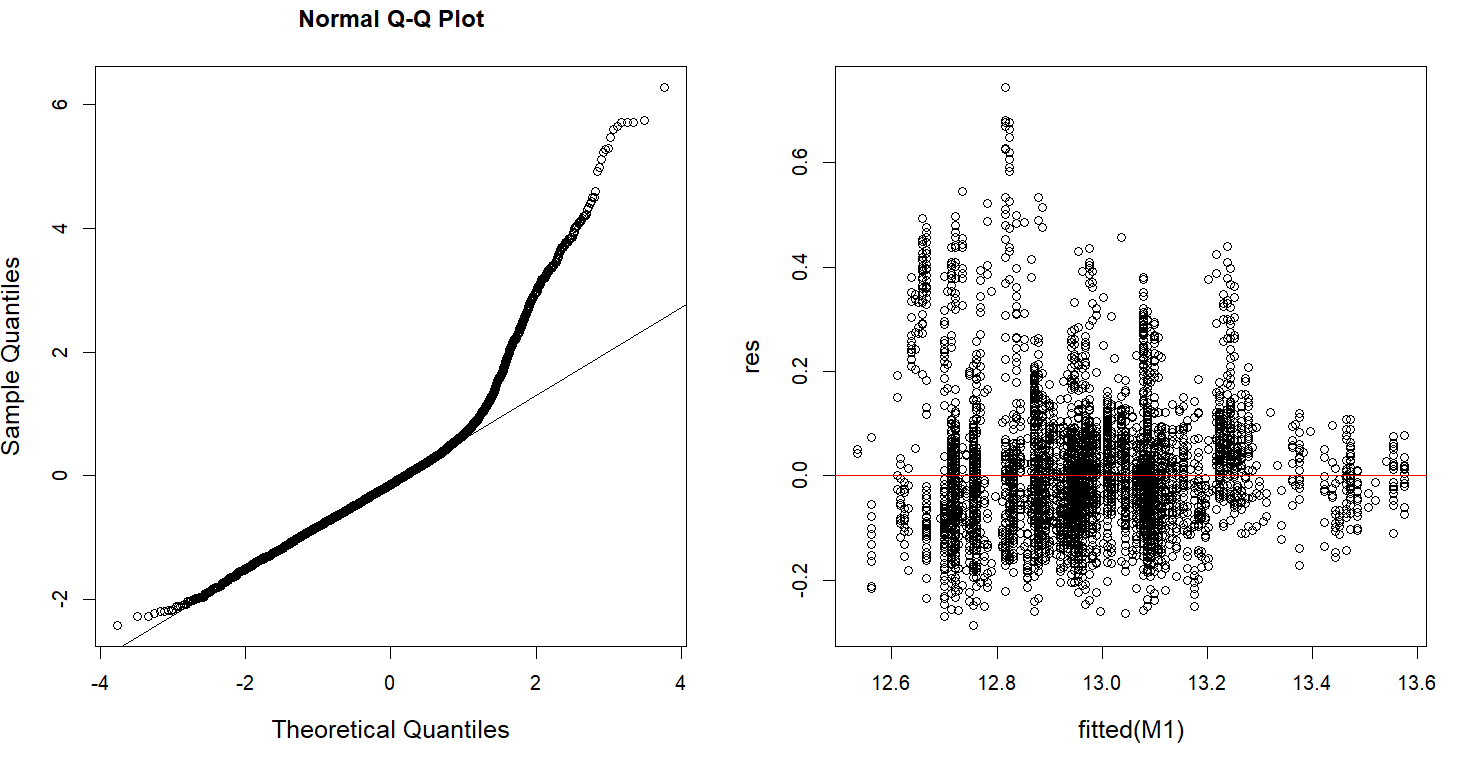
\includegraphics[width=0.9\textwidth]{images/Screenshot 2023-04-11 215131.png}
    \caption{Normal QQ-Plot and Residual Plot of $M_1$}
    \label{fig: m1 res plot and qq plot}
\end{figure}

\subsubsection{Intermediate Model}

Similarly, with the initial model, we apply a logarithm transform for the response variable \code{resale_price}.

Since the explanatory variables \code{floor_area_sqm} and \code{floor_area_sqft} are equivalent representations of each other (Fig. \ref{fig:scatterplot matrix}), we exclude \code{floor_area_sqft} to avoid multicollinearity in our model. We also exclude \code{flat_type} as there is some collinearity with \code{floor_area_sqm} (Fig. \ref{fig: boxplot}).

We include \code{flat_model} and \code{town} as categorical explanatory variables representing the model and location of the HDB flat respectively. These seem causally related to the resale price of the HDB flat so we included them.

We also include \code{storey_range}, a categorical explanatory variable to see if it would improve the model's fit and/or accuracy. Since \code{storey_range} has overlapping categories, we merge overlapping categories to encode. From this, 2 distinct categories are obtained, ``01 TO 15" and ``16 TO 27".

The interaction terms \code{floor_area_sqm * town}, \code{town * flat_model} and \code{flat_model * floor_area_sqm} were introduced to account for any interaction between these variables. Now the systematic component of the intermediate model includes the explanatory variables: \code{town}, \newline\code{floor_area_sqm}, \code{flat_model}, and \code{storey_range} and also the interaction terms mentioned above.
The intermediate model specification is as follows:
\begin{align*}
M2: \log(\text{resale\_price}) \sim \text{town} &+ \text{floor\_area\_sqm} + \text{flat\_model} + \text{storey\_range} + \text{floor\_area\_sqm * town} \\ &+ \text{town * flat\_model} + \text{flat\_model * floor\_area\_sqm}.
\end{align*}

\newpage

The model summary is given in Fig. \ref{fig: m2 model summary} and the fitted model equation is omitted here for conciseness (see Appendix).

\begin{figure}[!htp]
\centering
\begin{minipage}[t]{0.59\textwidth}
  \centering
    \caption{$M_2$ Model Summary}
    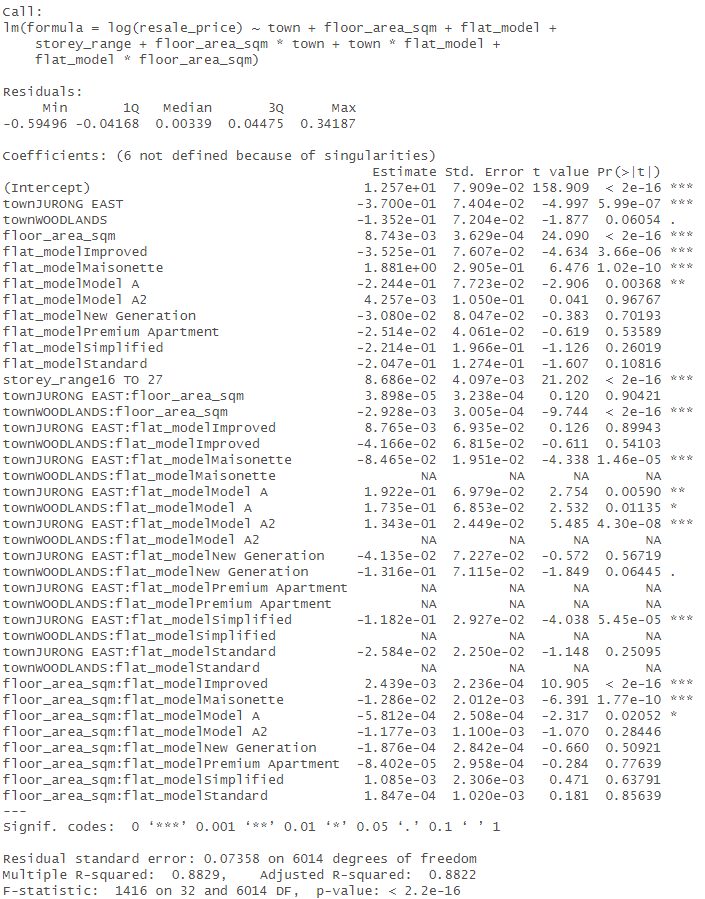
\includegraphics[width=\textwidth]{images2/Screenshot 2023-04-13 012323.png}
    \label{fig: m2 model summary}
\end{minipage}\hfill
\begin{minipage}[t]{0.37\textwidth}
  \centering
  \caption{$M_2$ Normal-QQ Plot and Residual Plot}
  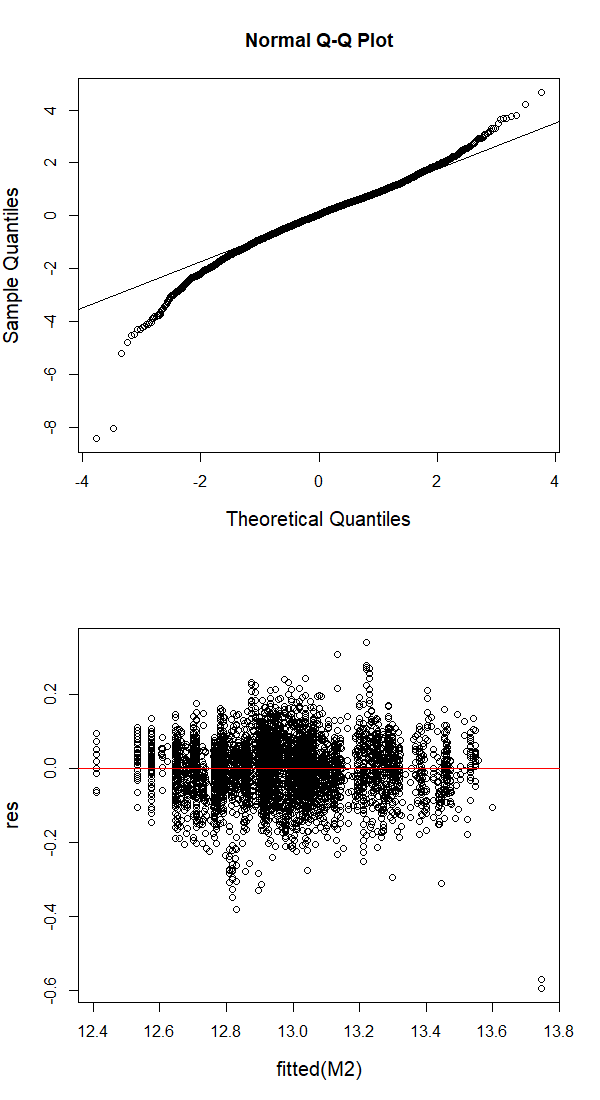
\includegraphics[width=\textwidth]{images2/m2updated.png}
  \label{fig: m2 assumption check}
\end{minipage}
\end{figure}
Like $M_1$, the p-value of the F-test ($<2.2 \times 10^{-16}$) for $M_2$ is very small and suggests that the overall model is statistically significant. Also, the adjusted $R^2$ value (0.8822) is high and improves significantly from $M_1$ (adjusted $R^2 = 0.694$). We compare the adjusted $R^2$ instead of multiple $R^2$ of $M_1$ and $M_2$ because it penalizes excessive model complexity and provides a more accurate measure of the proportion of variance in the dependent variable explained by the independent variables. This suggests that $M_2$ has stronger predictive power and better goodness-of-fit than $M_1$. The model also has a lower residual standard error of 0.07358 on 6014 degrees of freedom, improving from $M_1$.

Note that the normal QQ-plot of the SR of $M_2$ (Fig. \ref{fig: m2 assumption check}) shows the quantile points to be mostly consistent with the theoretical normal line. Hence, we conclude that the SR of $M_2$ do follow a normal distribution. Therefore, normality is present. From the residual plot (Fig, \ref{fig: m2 assumption check}) we observed that the spread of residuals across all levels of fitted values is more or less constant. Therefore, we conclude that the constant variance assumption holds. Since both normality and constant variance assumptions hold, $M_2$ is an accurate model.

Of the explanatory variables included, \code{town}, \code{floor_area_sqm}, \code{storey_range} are statistically significant, as indicated by the small p-values and *** in the model summary. The interaction terms \newline\code{flat_model * floor_area_sqm} and \code{town * flat_model} were not found to be statistically significant in $M_2$ and thus were discarded. However, the other interaction term \code{floor_area_sqm * town} was found to be significant, so we include it in our final model $M_n$.

\subsection{Final Model}
$M_n$ is specified:
\begin{align*}
    M_n : \log(\text{resale\_price}) \sim \text{town} &+ \text{floor\_area\_sqm} + \text{flat\_model} + \text{storey\_range} \\ &+ \text{floor\_area\_sqm * town} 
\end{align*}
The model summary is given in Fig. \ref{fig: mn model summary}.
\begin{figure}[!htp]
\centering
\begin{minipage}[t]{0.6\textwidth}
  \centering
    \caption{$M_n$ Model Summary}
    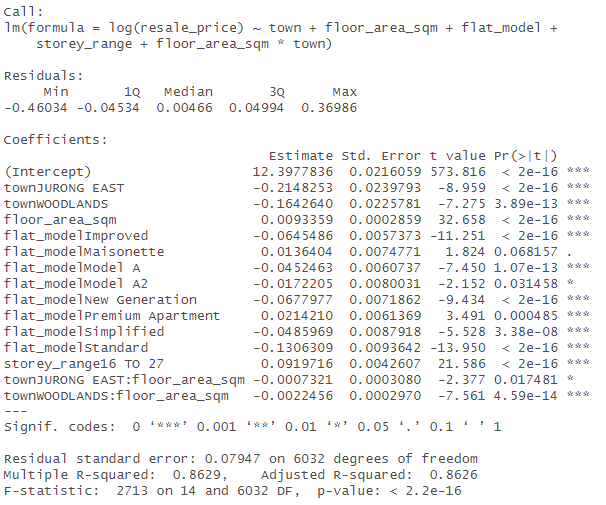
\includegraphics[width=\textwidth]{images2/Screenshot 2023-04-13 014027.png}
    \label{fig: mn model summary}
\end{minipage}\hfill
\begin{minipage}[t]{0.35\textwidth}
  \centering
  \caption{$M_n$ Normal-QQ Plot and Residual Plot}
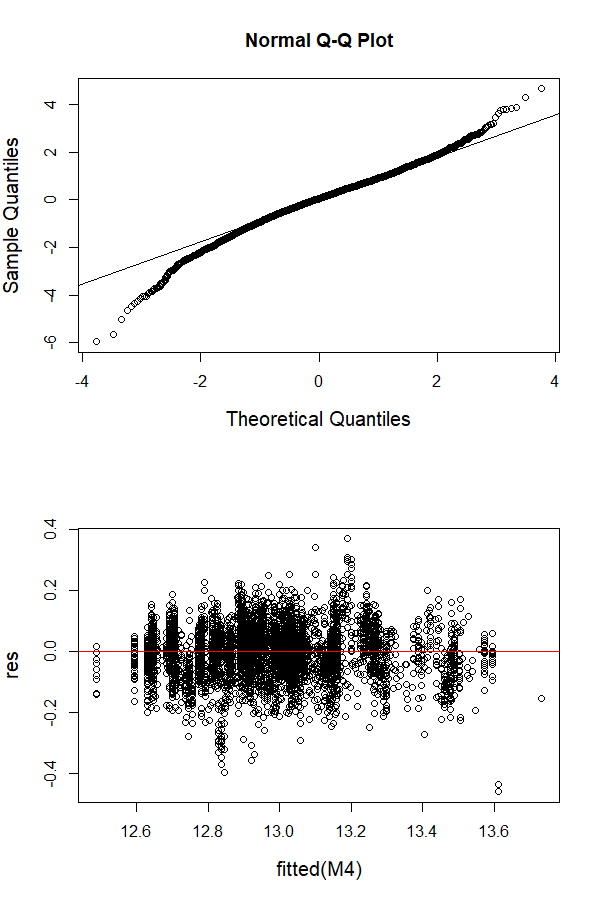
\includegraphics[width=\textwidth]{images2/mnupdated.png}
  \label{fig: mn assumption check}
\end{minipage}
\end{figure}
\newline
The model has an adjusted $R^2$ of 0.8626, indicating that the model explains 86.26\% of the variance in the log of resale price, after adjusting for the number of predictors. The residual standard error is 0.07947, suggesting that the model's predictions are, on average, within 7.95\% of the true log resale price. The adjusted $R^2$ value for $M_n$ is lower than the adjusted $R^2$ value for M2 (0.8822) but is still very high. Like M1 and M2, the p-value of the F-test ($ < 2.2 \times 10^{-16}$) for $M_n$ is very small, indicating that the overall model is statistically significant and has high goodness of fit. We prefer this model despite the slightly lower adjusted $R^2$ but with fewer regressors and interaction terms because it would have better generalization performance, meaning it would be less likely to overfit the training data and would better capture the true underlying relationship between the variables. Almost all of the regressors in M3 are statistically significant at the 99.9\% level as indicated by the p-value ($< 0.001$).

To check for normality and constant variance, we consider the normal QQ-plot of the SR of $M_n$ and the residual plot in Fig. \ref{fig: mn assumption check}. Note that the quantile points are very consistent with the theoretical normal line hence the SR of $M_n$ follow a normal distribution. So normality is present. From the residual plot, it is observed that the spread of residuals across all levels of fitted values is consistent. Therefore, we conclude that constant variance is present. Since the assumptions are satisfied, $M_n$ is an accurate model and therefore can be used. Finally, we check for outliers and influential points in R.
\begin{verbatim}
    > length(which(SR > 3 | SR < -3))
    [1] 52
    > C <- cooks.distance(Mn)
    > which(C > 1)
    named integer(0)
\end{verbatim}
The output tells us that there are 52 outliers (of 6047 observations) and no influential points as there are 0 points beyond the Cook's distance. Then the fitted equation for $M_n$ is given by:
\begin{align*}
    \log(\text{resale\_price}) &= 12.398 + 0.00934 * \text{floor\_area\_sqm} + 0.0920 * I(\text{storey\_range} = \text{16 TO 27})\\
    &-0.0645 * I(\text{flat\_model} = \text{Improved}) + 0.0136 * I(\text{flat\_model} = \text{Maisonette}) \\
    &-0.0452 * I(\text{flat\_model} = \text{Model A}) - 0.0172 * I(\text{flat\_model} = \text{Model A2}) \\
    &-0.0678 * I(\text{flat\_model} = \text{New Generation}) + 0.0214 * I(\text{flat\_model} = \text{Premium Apartment}) \\
    &-0.0486 * I(\text{flat\_model} = \text{Simplified}) - 0.131 * I(\text{flat\_model} = \text{Standard}) \\
    &+ I(\text{town} = \text{JURONG EAST})(-0.215 - 0.000732 \times\text{floor\_area\_sqm}) \\
    &+ I(\text{town} = \text{WOODLANDS})(-0.164 - 0.00225 \times \text{floor\_area\_sqm})
\end{align*}

The intercept coefficient is 12.398. This means that the mean value of \code{resale_price} of HDB flats is $e^{12.398} = 242,000$ when the floor area is 0 square metres, storey is within 1 to 15, flat model is Apartment, and location is CENTRAL AREA. Furthermore, the coefficient of indicator variable \code{storey_range} is 0.0920 so we expect, holding all other variables constant, the \code{resale_price} to be higher by $(e^{0.0920} - 1) \times 100 = 9.64\%$
The coefficient of \code{floor_area_sqm} is 0.00934. This means that for every 1 square meter increase in the floor area, the average percentage increase of the HDB flat \code{resale_price} is $(e^{0.00934} – 1) \times 100 = 0.938\%$ when the location is CENTRAL AREA and all other variables are held constant.
\\

The reference group is Apartment flats for analysis of \code{flat_model}. The coefficient is
\begin{enumerate}[noitemsep]
    \item -0.0645 when the flat model is Improved so we expect, holding all other variables constant, the mean \code{resale_price} to be lower by $(e^{-0.0645} - 1) \times 100 = -6.25$ \%
    \item +0.0136 when the flat model is Maisonette so we expect, holding all other variables constant, the mean \code{resale_price} to be higher by $(e^{0.0136} - 1) \times 100 = 1.37$ \%
    \item -0.0452 when the flat model is Model A so we expect, holding all other variables constant, the mean \code{resale_price} to be lower by $(e^{-0.0452} - 1) \times 100 = -4.42$ \%
    \item -0.0172 when the flat model is Model A2 so we expect, holding all other variables constant, the mean \code{resale_price} to be lower by $(e^{-0.0172} - 1) \times 100 = -1.71$ \%
    \item -0.0678 when the flat model is New Generation so we expect, holding all other variables constant, the mean \code{resale_price} to be lower by $(e^{-0.0678} - 1) \times 100 = -6.56$ \%
    \item +0.0214 when the flat model is Premium Apartment so we expect, holding all other variables constant, the mean \code{resale_price} to be higher by $(e^{0.0214} - 1) \times 100 = 2.16$ \%
    \item -0.0486 when the flat model is Simplified so we expect, holding all other variables constant, the mean \code{resale_price} to be lower by $(e^{-0.0486} - 1) \times 100 = -4.74$ \%
    \item -0.131 when the flat model is Standard so we expect, holding all other variables constant, the mean \code{resale_price} to be lower by $(e^{-0.131} - 1) \times 100 = -12.3$ \%
\end{enumerate}
when compared to HDBs of flat model Apartment.

For analysis of \code{town}, the reference group is flats in CENTRAL AREA. The coefficient of \code{town} is -0.215 and -0.164 when the flat is in JURONG EAST and WOODLANDS respectively. This means that we expect the mean \code{resale_price} to be lower by
\begin{enumerate}[noitemsep]
    \item $(e^{-0.215} - 1) \times 100 = -19.3\%$ on average for HDBs in JURONG EAST compared to CENTRAL AREA. 
    \item $(e^{-0.164} - 1) \times 100 = -15.1\%$ on average for HDBs in WOODLANDS compared to CENTRAL AREA.
\end{enumerate}
The coefficients for the interaction term \code{flat_model * floor_area_sqm} are -0.000732 and -0.00225. Hence, given a 1 square meter increase in \code{floor_area_sqm}, the average percentage increase in mean \code{resale_price} is $(e^{0.00934-0.000732} - 1) \times 100 = 0.865\%$ and $(e^{0.00934-0.00225} - 1) \times 100 = 0.712\%$ which is lower by $0.073\%$ and $0.226\%$ for flats in JURONG EAST and WOODLANDS, respectively, when compared to HDB flats in CENTRAL AREA.

\section{Conclusion}
In this analysis, we developed a linear regression model to predict HDB resale prices in Singapore. We started with a preliminary model that included several explanatory variables and iteratively refined the model through diagnostic tests and statistical analysis. Our final model includes significant regressors such as floor area, town, flat model, storey range, and the interaction terms between floor area and town, providing a good fit to the data with reasonable diagnostic results.

\end{document}